%\documentstyle[epsf,twocolumn]{jarticle}       %LaTeX2e仕様
\documentclass[twocolumn]{jarticle}     %pLaTeX2e仕様(platex.exeの場合)
%\documentclass[twocolumn]{ujarticle}     %pLaTeX2e仕様(uplatex.exeの場合)
%%%%%%%%%%%%%%%%%%%%%%%%%%%%%%%%%%%%%%%%%%%%%%%%%%%%%%%%%%%%%%
%%
%%  基本バージョン
%%
%%%%%%%%%%%%%%%%%%%%%%%%%%%%%%%%%%%%%%%%%%%%%%%%%%%%%%%%%%%%%%%%
\setlength{\topmargin}{-45pt}
%\setlength{\oddsidemargin}{0cm} 
\setlength{\oddsidemargin}{-7.5mm}
%\setlength{\evensidemargin}{0cm} 
\setlength{\textheight}{24.1cm}
%setlength{\textheight}{25cm} 
\setlength{\textwidth}{17.4cm}
%\setlength{\textwidth}{172mm} 
\setlength{\columnsep}{11mm}

\kanjiskip=.07zw plus.5pt minus.5pt


% 【節が変わるごとに (1.1)(1.2) … (2.1)(2.2) と数式番号をつけるとき】
%\makeatletter
%\renewcommand{\theequation}{%
%\thesection.\arabic{equation}} %\@addtoreset{equation}{section}
%\makeatother

%\renewcommand{\arraystretch}{0.95} 行間の設定

%%%%%%%%%%%%%%%%%%%%%%%%%%%%%%%%%%%%%%%%%%%%%%%%%%%%%%%%
\usepackage[dvipdfmx]{graphicx}   %pLaTeX2e仕様(\documentstyle ->\documentclass)\documentclass[dvipdfmx]{graphicx}
\usepackage[dvipdfmx]{color}
\usepackage[subrefformat=parens]{subcaption}
\usepackage{colortbl}
\usepackage{multicol}
%%%%%%%%%%%%%%%%%%%%%%%%%%%%%%%%%%%%%%%%%%%%%%%%%%%%%%%%

\begin{document}

\twocolumn[
\noindent

\hspace{1em}
2020年11月13日
\hfill
\ \ 細川 岳大

\vspace{2mm}

\hrule

\begin{center}
{\Large \bf 進捗報告}
\end{center}
\hrule
\vspace{3mm}
]

% ‚ここから 文章 Start!

\section{今週やったこと}

\begin{itemize}
	%\item optuna
	\item 予測精度の実験
	\item GAの実験
\end{itemize}

\section{精度とランダムラベルの割合}
前回のランダムラベルでの実験について再度検証を行った.
表\ref{tb:SVMpara}に設定を示す.
また,この設定は先週の実験でoptunaで探索したものである\\.
各割合に対し,50回ずつ実験を行った.
\begin{table}[h]
	\centering
	\caption{SVMの設定\label{tb:SVMpara}}
	\scalebox{1.0}{
		\begin{tabular}{|c|c|} \hline
			kernel&poly\\ \hline
			C&3.654\\ \hline
			$\gamma$&53.15\\ \hline
			coef0&0.0\\ \hline
			degree&3\\ \hline\hline
			dataset&cifar10\\ \hline
			train&200\\ \hline
			test&200\\ \hline
		\end{tabular}
	}
\end{table}

\subsection{結果}
表\ref{tb:res1}に結果を示す.
結果としてはランダムなものが少ないほど精度は高く,かなり妥当なものであることが分かる.

\begin{table}[h]
	\centering
	\caption{結果\label{tb:res1}}
	\scalebox{1.0}{
		\begin{tabular}{|c|c|} \hline
			random&accuracy\\ \hline
			0&0.2538$\pm$0.0344\\ \hline
			1&0.2523$\pm$0.0344\\ \hline
			2&0.2526$\pm$0.0364\\ \hline
			4&0.2514$\pm$0.0314\\ \hline
			8&0.2510$\pm$0.0300\\ \hline
			16&0.2390$\pm$0.0323\\ \hline
			32&0.2245$\pm$0.0329\\ \hline
			64&0.1989$\pm$0.0286\\ \hline
			128&0.1499$\pm$0.0309\\ \hline
		\end{tabular}
	}
\end{table}

\section{GAの実験}

ラベルなし画像100枚取り出し,それらに対するラベルをGAによって探索する.
表\ref{tb:GApara}に実験の設定を示す.
SVMのハイパーパラメータはoptunaで最適化した.今回はランダムなラベルの数と精度に対する相関係数
を目的関数とした.
遺伝子は0から9の整数値をとる整数値コーディングとした.\\
選択はサイズ2のトーナメント選択,交叉には二点交叉,突然変異は別の数値にランダムに移るように設定した.\\
前回との変更点として,データの前処理を正規化から標準化にした.
また,前回trainとevalの分け方を世代ごとに変えるということをしていたが,
それだけでは世代ごとの適応度のばらつきがあったので,今回はさらに5回の試行の平均を適応度とした.

\begin{table}[h]
	\centering
	\caption{GAの設定\label{tb:GApara}}
	\scalebox{1.0}{
		\begin{tabular}{|c||c|} \hline
			個体数&30\\ \hline
			世代数&100\\ \hline
			交叉率&1.0\\ \hline
			突然変異率&0.02\\ \hline\hline
			全ラベル付き画像&250枚\\ \hline
			train:eval&100枚:150枚\\ \hline
			search&100枚\\ \hline
		\end{tabular}
	}
\end{table}

\subsection{実験2.1}
最適化関数の相関係数を求めるにあたり,
250枚のラベル付き画像をtrain:testを150枚:100枚に分け,
trainのうちランダムなラベル数を0,1,4,9,16,25,36,49,64,128と変化させ,
各20回ずつ試行した.
こうして得られた精度とそれに対するランダムなラベル数の相関係数を最適化関数とした.
またoptunaの試行回数は200回とした.
表\ref{tb:SVM1para}に探索したパラメータ及びその時の相関係数を示す.

\begin{table}[h]
	\centering
	\caption{実験2.1のSVMのパラメータ\label{tb:SVM1para}}
	\scalebox{1.0}{
		\begin{tabular}{|c|c|c|} \hline
			\multicolumn{2}{|c|}{探索}&best\\ \hline
			kernel&rbf, sigmoid, poly, linear&poly\\ \hline
			C&$10^{-1}$ - $10^{3}$&799.7\\ \hline
			$\gamma$&$10^{-4}$ - $10^{2}$&$9.494*10^{-2}$\\ \hline
			coef0&$10^{-1}$ - $10$&0.9060\\ \hline\hline
			\multicolumn{2}{|c|}{固定}&\\ \hline
			\multicolumn{2}{|c|}{degree}&3\\ \hline\hline
			\multicolumn{2}{|c|}{相関係数}&0.6833\\ \hline
		\end{tabular}
	}
\end{table}


\subsection{実験2.2}
最適化関数の相関係数を求めるにあたり,
250枚のラベル付き画像をtrain:testを125枚:125枚に分け,
trainのうちランダムなラベル数を100から119と変化させ,
各20回ずつ試行した.
こうして得られた精度とそれに対するランダムなラベル数の相関係数を最適化関数とした.
またoptunaの試行回数は200回とした.
表\ref{tb:SVM2para}に探索したパラメータ及びその時の相関係数を示す.

\begin{table}[h]
	\centering
	\caption{実験2.2のSVMのパラメータ\label{tb:SVM2para}}
	\scalebox{1.0}{
		\begin{tabular}{|c|c|c|} \hline
			\multicolumn{2}{|c|}{探索}&best\\ \hline
			kernel&rbf, sigmoid, poly, linear&linear\\ \hline
			C&$10^{-1}$ - $10^{3}$&821.3\\ \hline
			$\gamma$&$10^{-4}$ - $10^{2}$&$2.285*10^{-4}$\\ \hline
			coef0&$10^{-1}$ - $10$&1.308\\ \hline\hline
			\multicolumn{2}{|c|}{固定}&\\ \hline
			\multicolumn{2}{|c|}{degree}&3\\ \hline\hline
			\multicolumn{2}{|c|}{相関係数}&0.3265\\ \hline
		\end{tabular}
	}
\end{table}



\subsection{結果}
図\ref{fig:ex1},\ref{fig:ex2}に結果を示す.
前回に比べ適応度のばらつきは押さえられていた.
また,相関係数が示すようにSVMで全域的には相関関係があり,
ランダムなラベルが多い局所的な箇所では相関関係がないといえる.


\begin{figure}[h]
	\begin{center}
		\vspace*{-7mm}
		\hspace*{-8mm}
		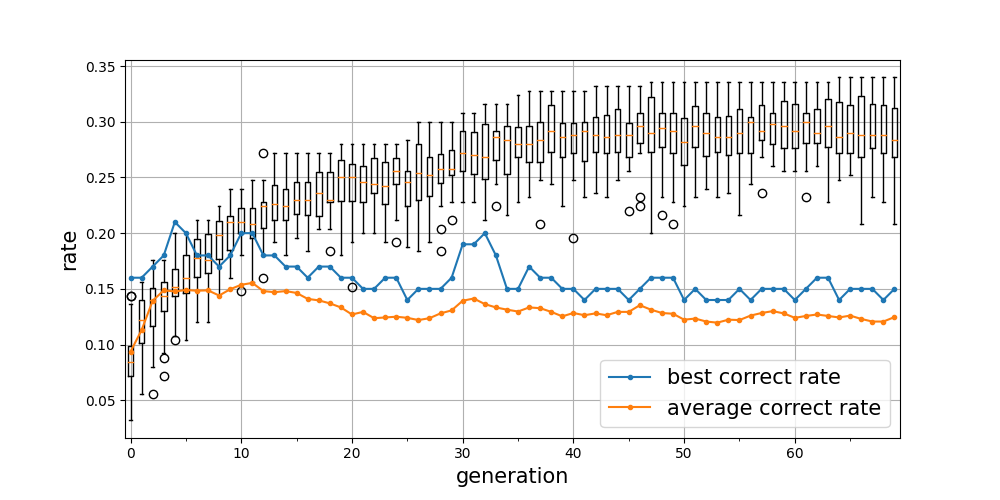
\includegraphics[height=65mm,width=110mm]{graph_1.png}
		\caption{実験2.1の結果\label{fig:ex1}}
	\end{center}
\end{figure}

\begin{figure}[h]
	\begin{center}
		\vspace*{-7mm}
		\hspace*{-8mm}
		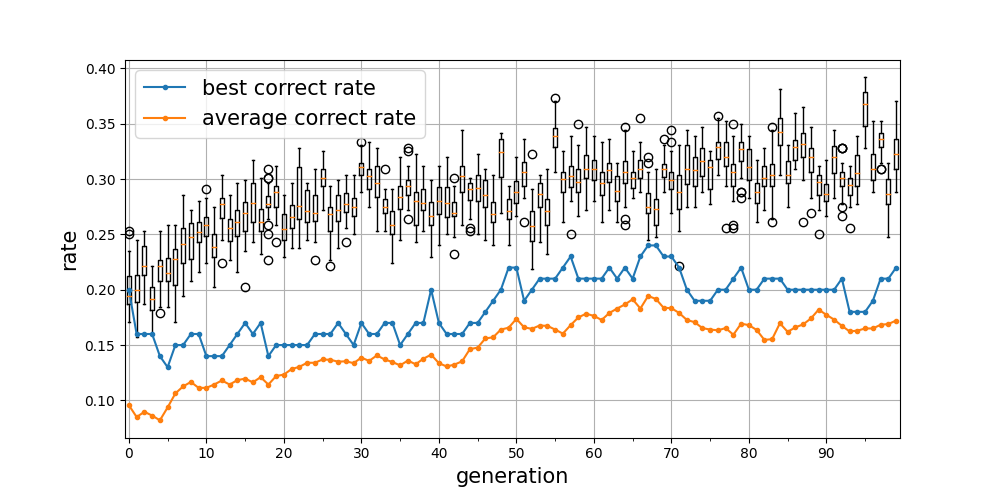
\includegraphics[height=65mm,width=110mm]{graph_2.png}
		\caption{実験2.2の結果\label{fig:ex2}}
	\end{center}
\end{figure}

\section{来週の課題}
	\begin{itemize}
		\item GAをFixMatchを用いて探索中
	\end{itemize}


\end{document}


